\documentclass[11pt,reqno]{amsart}
\usepackage[top=1in, left=1in, right=1in, bottom=1in]{geometry}                % See geometry.pdf to learn the layout options. There are lots.
\geometry{letterpaper}                   % ... or a4paper or a5paper or ...
\usepackage[parfill]{parskip}    % Activate to begin paragraphs with an empty line rather than an indent
%\usepackage{algorithm}

\usepackage{algorithm}
\usepackage{algpseudocode}

\usepackage{graphicx}

\usepackage{verbatim}
\usepackage{amssymb}
\usepackage{amsmath}

\usepackage{enumitem}

\usepackage{setspace}
\doublespacing

\usepackage{natbib}

%\usepackage{epstopdf}
%\DeclareGraphicsRule{.tif}{png}{.png}{`convert #1 `dirname #1`/`basename #1 .tif`.png}

\newcommand{\RR}{I\!\!R} %real numbers
\DeclareMathOperator{\diag}{diag}

\algnewcommand{\Inputs}[1]{%
  \State \textbf{Inputs:}
  \Statex \hspace*{\algorithmicindent}\parbox[t]{.8\linewidth}{\raggedright #1}
}
\algnewcommand{\Initialize}[1]{%
  \State \textbf{Initialize:}
  \Statex \hspace*{\algorithmicindent}\parbox[t]{.8\linewidth}{\raggedright #1}
}

\title[RVD2]{Variational Inference on RVD2 model}
\author{Y. He}
\date{}                                           % Activate to display a given date or no date

\begin{document}

\maketitle


%%%%%%%%%%%%%%%%%%
% Model Structure
%%%%%%%%%%%%%%%%%%
\section{Model Structure}\label{sec:model_structure}




\begin{figure}[h]
\begin{center}
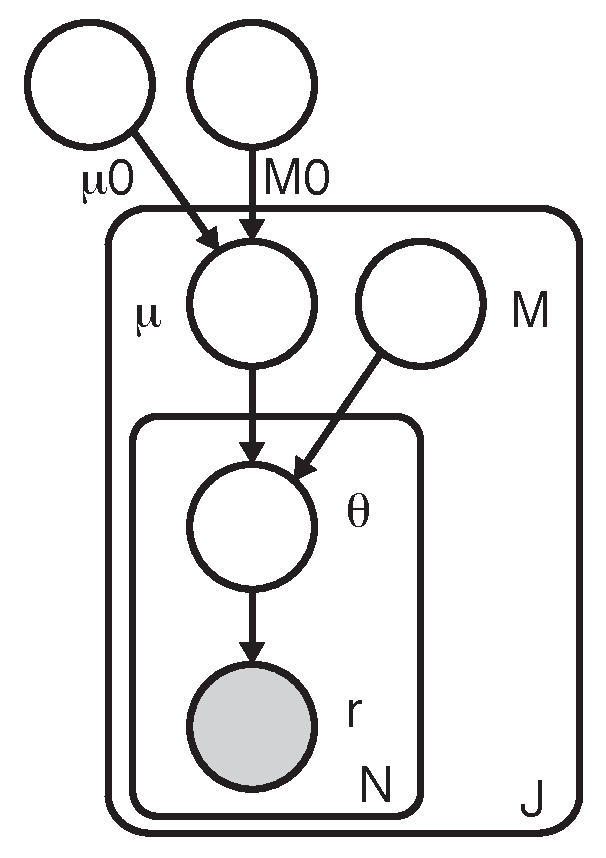
\includegraphics[width=40mm]{pdf_figs/RVD2_model.pdf}
\caption{RVD2 Graphical Model}
\label{fig:graphical_model}
\end{center}
\end{figure}


The joint distribution over the latent and observed variables for data at location $j$ in replicate $i$ given the parameters is

\begin{equation}\label{eqn:jointpdf}
p \left( r_{ji}, \theta_{ji}, \mu_j | n_{ji}; \mu_0, M_0, M_j \right) = p \left( r_{ji} | \theta_{ji}, n_{ji} \right) p\left( \theta_{ji} | \mu_j; M_j \right) p\left( \mu_j; \mu_0, M_0 \right),
\end{equation}

where
\begin{align}
p\left( \mu_j; \mu_0, M_0 \right)  &= \frac{ \Gamma(M_0) } { \Gamma(\mu_0 M_0) \Gamma(M_0 (1-\mu_0)) } \mu_j^{M_0\mu_0 -1} (1 - \mu_j)^{M_0 ( 1 - \mu_0) - 1}, \nonumber \\
p\left( \theta_{ji} | \mu_j; M_j \right) &= \frac{ \Gamma(M_j) } { \Gamma(\mu_j M_j) \Gamma(M_j (1-\mu_j)) } \theta_{ji}^{M_j\mu_j -1} (1 - \theta_{ji})^{M_j ( 1 - \mu_j) - 1}, \nonumber \\
p \left( r_{ji} | \theta_{ji}, n_{ji} \right) &= \frac{ \Gamma(n_{ji}+1) } { \Gamma(r_{ji}+1) \Gamma( n_{ji} - r_{ji} + 1 ) } \theta_{ji}^{r_{ji}} (1 - \theta_{ji})^{n_{ji} - r_{ji}}. \nonumber
\end{align}

Integrating over the latent variables $\theta_{ji}$ and $\mu_j$ yields the marginal distribution of the data,
\begin{equation}
p \left( r_{ji} | n_{ji} ; \mu_0, M_0, M_j \right) = \int_{\mu_j} \int_{\theta_{ji}}  p \left( r_{ji} | \theta_{ji}, n_{ji} \right) p\left( \theta_{ji} | \mu_j; M_j \right) p\left( \mu_j; \mu_0, M_0 \right) d\theta_{ji} d\mu_j.
\end{equation}

Finally, the log-likelihood of the data set is

\begin{equation}
\log p \left( r | n ; \mu_0, M_0, M \right) = \sum_{j=1}^J \sum_{i=1}^N \log \int_{\mu_j} \int_{\theta_{ji}}  p \left( r_{ji} | \theta_{ji}, n_{ji} \right) p\left( \theta_{ji} | \mu_j; M_j \right) p\left( \mu_j; \mu_0, M_0 \right) d\theta_{ji} d\mu_j.
\end{equation}



%%%%%%%%%%%%%%%%%%
% Variational approach
%%%%%%%%%%%%%%%%%%
\section{Variational Inference}

\subsection{Factorization} 

We propose the following factorized variational distribution to approximate the true posterior over latent variables:
\begin{equation}
  q(\mu, \theta) = q(\mu)q(\theta) = \prod_{j=1}^J q(\mu_{j}) \prod_{i=1}^N q(\theta_{ji}).
  \label{eq:vardist}
\end{equation}


\subsection{Derivation of $ q(\mu) $ and $ q(\theta) $}

\subsubsection{Derivation of $ q(\theta) $} Taking the expectation of the complete log likelihood over all variables except $ \theta$, the "best" distribution $ q_\theta^*(\theta) $ can be represented as
\begin{equation}
\begin{split}
\log q_\theta^*(\theta) &= E_\mu\left[ \log p\left(r,\mu,\theta | n; \phi \right) \right] \\
&= E_\mu \left[ \log p\left(r | \theta, n \right)\right] + E_\mu \left[ \log p\left(\theta | \mu; M \right)\right] + E_\mu \left[ \log p\left(\mu ; \mu_0, M_0 \right)\right] \\
&= \sum_{j=1}^{J} \sum_{i=1}^{N} E_\mu  \left[ \log p \left( r_{ji} | \theta_{ji}, n_{ji} \right) \right] + \sum_{j=1}^{J} \sum_{i=1}^{N} E_\mu \left[ \log p\left(\theta_{ji} | \mu_j; M_j \right)\right] + \sum_{j=1}^{J} E_\mu \left[ \log p\left(\mu_j | \mu_0; M_0 \right)\right] \\
\end{split}
\end{equation}

Leaving out the items not depending on $\theta$ gives,
\begin{equation}
\begin{split}
\log q_\theta^*(\theta) &\propto E_\mu \left[ \log p\left(r | \theta, n \right)\right] + E_\mu \left[ \log p\left(\theta | \mu; M \right)\right] \\
&\propto \sum_{j=1}^{J} \sum_{i=1}^{N} E_\mu  \left[ \log p \left( r_{ji} | \theta_{ji}, n_{ji} \right) \right] + \sum_{j=1}^{J} \sum_{i=1}^{N} E_\mu \left[ \log p\left(\theta_{ji} | \mu_j; M_j \right)\right] \\
&\propto \sum_{j=1}^{J} \sum_{i=1}^{N}  E_\mu  \left[ \log \left( \frac{ \Gamma(n_{ji}+1) } { \Gamma(r_{ji}+1) \Gamma( n_{ji} - r_{ji} + 1 ) } \theta_{ji}^{r_{ji}} (1 - \theta_{ji})^{n_{ji} - r_{ji}} \right) \right] \\
&\quad + \sum_{j=1}^{J} \sum_{i=1}^{N}  E_\mu  \left[ \log \left( \frac{ \Gamma(M_j) } { \Gamma(\mu_j M_j) \Gamma(M_j (1-\mu_j)) } \theta_{ji}^{M_j\mu_j -1} (1 - \theta_{ji})^{M_j ( 1 - \mu_j) - 1} \right) \right] \\
&\propto \sum_{j=1}^{J} \sum_{i=1}^{N} E_\mu\left[ \log \left( \theta_{ji}^{r_{ji} + M_j\mu_j -1} (1 - \theta_{ji})^{n_{ji} - r_{ji} + M_j ( 1 - \mu_j) - 1} \right) \right] \\
&\propto  \sum_{j=1}^{J} \sum_{i=1}^{N} \log \left( \theta_{ji}^{r_{ji} + M_j E_{\mu_j}\left[ \mu_j\right] -1} (1 - \theta_{ji})^{n_{ji} - r_{ji} + M_j ( 1 - E_{\mu_j}\left[ \mu_j\right]) - 1} \right) \\
\end{split}
\end{equation}

Exponentiating both sides, we can see that  $ q_\theta^*(\theta) $ is a product of beta distributions. The optimal variational distribution for $ \theta_{ji} $ is Beta distribution.
\iffalse
\begin{align}
\theta_{ji} \thicksim \text{Binomial}(\alpha_{ji}, \beta_{ji})
\end{align}
where,
\begin{align}
\alpha_{ji} &= r_{ji} + M_j E_\mu\left[ \mu_j\right] -1 \nonumber \\
\beta_{ji} &= n_{ji} - r_{ji} + M_j ( 1 - E_\mu\left[ \mu_j\right]) \nonumber
\end{align}
\fi

 

\subsubsection{Derivation of $ q(\mu) $}
Taking the expectation of the complete log likelihood over all variables except $ \mu $, the "best" distribution $ q_\mu^*(\mu) $ can be represented as
\begin{equation}
\begin{split}
\log q_\mu^*(\mu) &= E_\theta\left[ \log p\left(r,\mu,\theta | n; \phi \right) \right] \\
&= E_\theta \left[ \log p\left(r | \theta, n \right)\right] + E_\theta \left[ \log p\left(\theta | \mu; M \right)\right] + E_\theta \left[ \log p\left(\mu ; \mu_0, M_0 \right)\right] \\
\end{split}
\end{equation}

Leaving out the items not depending on $\mu$ gives,

\begin{equation}
\begin{split}
\log q_\mu^*(\mu) &\propto \sum_{j=1}^{J} \sum_{i=1}^{N} E_\theta \left[ \log p\left(\theta_{ji} | \mu_j; M_j \right)\right] + \sum_{j=1}^{J} E_\theta  \left[ \log p\left( \mu_j; \mu_0, M_0 \right) \right] \\
&\propto \sum_{j=1}^{J} \sum_{i=1}^{N}  E_\theta  \left[ \log \left( \frac{ \Gamma(M_j) } { \Gamma(\mu_j M_j) \Gamma(M_j (1-\mu_j)) } \theta_{ji}^{M_j\mu_j -1} (1 - \theta_{ji})^{M_j ( 1 - \mu_j) - 1} \right) \right] \\
&\quad + \sum_{j=1}^{J} E_\theta  \left[ \log \left( \frac{ \Gamma(M_0) } { \Gamma(\mu_0 M_0) \Gamma(M_0 (1-\mu_0)) } \mu_j^{M_0\mu_0 -1} (1 - \mu_j)^{M_0 ( 1 - \mu_0) - 1} \right) \right] \\
&\propto \sum_{j=1}^{J} - \log \Gamma(\mu_j M_j)  - \log \Gamma(M_j (1-\mu_j)) + \sum_{j=1}^{J} \sum_{i=1}^{N} M_j\mu_j \left\lbrace   E_\theta  \left[ \log \theta_{ji}\right] - E_\theta  \left[ \log \left( 1- \theta_{ji}\right) \right] \right\rbrace \\
&\quad + \sum_{j=1}^{J} \left\lbrace (M_0 \mu_0 - 1) \log \mu_j + (M_0 ( 1 - \mu_0) - 1) \log ( 1 - \mu_j)\right\rbrace \\
\end{split}
\end{equation}

It can be seen that the distribution function of $ q_\mu^*(\mu) $ is not any known distribution. We propose to approximate $ q_\mu^*(\mu) $ using Laplace approximation  distribution.

\begin{align}
\mu_j \thicksim \mathcal{N}(\hat{\mu}_j, {-f''(\hat{\mu}_j ) }^{-1})
\end{align}

Where $ \hat{\mu}_j $ is the stationary point which maximize the ELBO, and $ f(\mu_j) $ isolates all the terms involves $ \mu_j $. As $ \mu_j $ is within $ [0,1] $, $ \mu_j $ follows a truncated normal distribution.

Isolating items in $ \log q_\mu^*(\mu) $ that depends on $ \mu_j $ gives

\begin{equation}
\begin{split}
f(\mu_j)
&= - \log \Gamma(\mu_j M_j) - \log \Gamma(M_j (1-\mu_j))\\
&\quad + \sum_{i=1}^{N} M_j\mu_j \left\lbrace   E_\theta  \left[ \log \theta_{ji}\right] - E_\theta  \left[ \log \left( 1- \theta_{ji}\right) \right] \right\rbrace \\
&\quad + \left\lbrace (M_0 \mu_0 - 1) \log \mu_j + (M_0 ( 1 - \mu_0) - 1) \log ( 1 - \mu_j)\right\rbrace \\
\end{split}
\end{equation}

Take the first derivative with respect to $ \mu_j $,

\begin{equation}
\label{f''(mu)}
\begin{split}
%\frac{\partial f(\mu_j)}{\partial \mu_j}
f'(\mu_j) &= -M_j\psi (\mu_j M_j) + M_j \psi (M_j(1-\mu_j))\\
&\quad + \sum_{i=1}^{N} M_j \left\lbrace   E_\theta  \left[ \log \theta_{ji}\right] - E_\theta  \left[ \log \left( 1- \theta_{ji}\right) \right] \right\rbrace\\
&\quad + \left\lbrace \frac{M_0 \mu_0 - 1}{\mu_j} - \frac{M_0 ( 1 - \mu_0) - 1}{ 1 - \mu_j} \right\rbrace \\
\end{split}
\end{equation}

The second derivative with respect to $ \mu_j $ is,
\begin{equation}
\begin{split}
%\frac{\partial^2 f(\mu_j)}{\partial \mu_j ^2} 
f''(\mu_j)&= -M_j^2\psi' (\mu_j M_j) - M_j^2 \psi' (M_j(1-\mu_j))\\
&\quad + \left\lbrace \frac{1 - M_0 \mu_0}{\mu_j^2} - \frac{M_0 ( 1 - \mu_0) - 1}{ (1 - \mu_j)^2} \right\rbrace \\
\end{split}
\end{equation}

where $ \psi(\mu) $ is the Digamma function, and $ \psi'(\mu)= \frac{\partial \psi(\mu)}{\partial \mu}$ is the Trigamma function.
\subsection{ELBO compute}

Using Jensen's inequality, the log-likelihood of the data is lower-bounded:

\begin{equation}
\begin{split}
\log p \left( r | \phi \right) &= \log \int_\mu \int_\theta p\left(r,\mu,\theta \right) d\theta d\mu \\ 
&= \log \int_\mu \int_\theta p\left(r,\mu,\theta \right)\frac{q\left(\mu,\theta \right) }{q\left(\mu,\theta \right) } d\theta d\mu \\ 
&\geq \int_\mu \int_\theta q\left(\mu,\theta \right) \log \frac{ p\left(r,\mu,\theta \right)}{q\left(\mu,\theta \right)} d\theta d\mu \\
&= E_q \left[ \log p\left(r,\mu,\theta \right)\right] - E_q \left[ \log q\left(\mu,\theta \right)\right] \\
&\triangleq \mathcal{L}(q, \phi) ,
\end{split}
\end{equation}

where $ \phi= \left( \mu_0, M_0, M \right) $

Actually, 

\begin{equation}
\begin{split}
\log p \left( r | \phi \right) &= \log \int_\mu \int_\theta p\left(r,\mu,\theta \right) d\theta d\mu \\ 
&= \log \int_\mu \int_\theta p\left(r,\mu,\theta \right)\frac{q\left(\mu,\theta \right) }{q\left(\mu,\theta \right) } d\theta d\mu \\ 
&= \int_\mu \int_\theta q\left(\mu,\theta \right) \log \frac{ p\left(r,\mu,\theta \right)}{q\left(\mu,\theta \right)} d\theta d\mu - \int_\mu \int_\theta q\left(\mu,\theta \right) \log \dfrac{p\left( \mu, \theta | r\right) }{q\left(\mu,\theta \right)} d\theta d\mu \\
&= \mathcal{L}(q, \phi) + KL\left(q(\mu,\theta ) || p( \mu, \theta | r) \right) ,
\end{split}
\end{equation}

Maximizing the ELBO is equivalent to minimizing the KL-divergence between the variational distribution and the true posterior.


Writing out ELBO $ \mathcal{L}(q, \phi) $, we have
\begin{equation}
\begin{split}
\label{L}
\mathcal{L}(q, \phi) &= E_q \left[ \log p\left(r,\mu,\theta | n; \phi \right)\right] - E_q \left[ \log q\left(\mu,\theta \right)\right] \\
&= E_q \left[ \log p\left(r | \theta, n \right)\right] + E_q \left[ \log p\left(\theta | \mu; M \right)\right] + E_q \left[ \log p\left(\mu ; \mu_0, M_0 \right)\right]- E_q \left[ \log q\left(\mu \right)\right]- E_q \left[ \log q\left(\theta \right)\right] \\
\end{split}
\end{equation}

\begin{equation}
\begin{split}
\label{r}
E_q \left[ \log p\left(r | \theta, n \right)\right] &= \sum_{j=1}^{J} \sum_{i=1}^{N} E_q  \left[ \log p \left( r_{ji} | \theta_{ji}, n_{ji} \right) \right] \\
&= \sum_{j=1}^{J} \sum_{i=1}^{N}  E_q  \left[ \log \left( \frac{ \Gamma(n_{ji}+1) } { \Gamma(r_{ji}+1) \Gamma( n_{ji} - r_{ji} + 1 ) } \theta_{ji}^{r_{ji}} (1 - \theta_{ji})^{n_{ji} - r_{ji}} \right) \right] \\
%&= \sum_{j=1}^{J} \sum_{i=1}^{N}  E_q  \left[ r_{ji} \log \theta_{ji} + (n_{ji} - r_{ji}) \log (1 - \theta_{ji}) \right] + con. \\
%&= \sum_{j=1}^{J} \sum_{i=1}^{N} \left\lbrace r_{ji} E_q \left[ \log \theta_{ji} \right] + (n_{ji} - r_{ji}) E_q  \left[  \log (1 - \theta_{ji}) \right] \right\rbrace + con. \\
%
&= \sum_{j=1}^{J} \sum_{i=1}^{N} \log \left( \frac{ \Gamma(n_{ji}+1) } { \Gamma(r_{ji}+1) \Gamma( n_{ji} - r_{ji} + 1 ) }\right)  \\
&\quad + \sum_{j=1}^{J} \sum_{i=1}^{N}  E_q  \left[ r_{ji} \log \theta_{ji} + (n_{ji} - r_{ji}) \log (1 - \theta_{ji}) \right] \\
&= \sum_{j=1}^{J} \sum_{i=1}^{N} \log \left( \frac{ \Gamma(n_{ji}+1) } { \Gamma(r_{ji}+1) \Gamma( n_{ji} - r_{ji} + 1 ) }\right)  \\
&\quad + \sum_{j=1}^{J} \sum_{i=1}^{N} \left\lbrace r_{ji} E_q \left[ \log \theta_{ji} \right] + (n_{ji} - r_{ji}) E_q  \left[  \log (1 - \theta_{ji}) \right] \right\rbrace \\
\end{split}
\end{equation}

\begin{equation}
\begin{split}
\label{theta}
E_q \left[ \log p\left(\theta | \mu; M \right)\right] &= \sum_{j=1}^{J} \sum_{i=1}^{N} E_q \left[ \log p\left(\theta_{ji} | \mu_j; M_j \right)\right] \\
&= \sum_{j=1}^{J} \sum_{i=1}^{N}  E_q  \left[ \log \left( \frac{ \Gamma(M_j) } { \Gamma(\mu_j M_j) \Gamma(M_j (1-\mu_j)) } \theta_{ji}^{M_j\mu_j -1} (1 - \theta_{ji})^{M_j ( 1 - \mu_j) - 1} \right) \right] \\
%
&= \sum_{j=1}^{J} E_q  \left[ \log \left( \frac{ \Gamma(M_j) } { \Gamma(\mu_j M_j) \Gamma(M_j (1-\mu_j)) }\right) \right] + \sum_{j=1}^{J} \sum_{i=1}^{N}  E_q  \left[ \log \left( \theta_{ji}^{M_j\mu_j -1} (1 - \theta_{ji})^{M_j ( 1 - \mu_j) - 1} \right) \right] \\
%
&= \sum_{j=1}^{J} E_q  \left[ \log \left( \frac{ \Gamma(M_j) } { \Gamma(\mu_j M_j) \Gamma(M_j (1-\mu_j)) }\right) \right]  \\ 
&\quad + \sum_{j=1}^{J} \sum_{i=1}^{N} \left\lbrace E_q \left[ \left( M_j\mu_j -1 \right) \log \theta_{ji} \right] + E_q \left[ \left( M_j ( 1 - \mu_j) - 1 \right) \log \left( 1 - \theta_{ji} \right) \right]\right\rbrace \\
%
&= \sum_{j=1}^{J} E_q  \left[ \log \left( \frac{ \Gamma(M_j) } { \Gamma(\mu_j M_j) \Gamma(M_j (1-\mu_j)) }\right) \right] \\ 
&\quad + \sum_{j=1}^{J} \sum_{i=1}^{N} \left\lbrace M_j E_q \left[ \mu_j \right] E_q \left[ \log \theta_{ji} \right] - E_q  \left[ \log \theta_{ji} \right] + \left( M_j - 1 - M_j E_q\left[ \mu_j \right]  \right) E_q\left[ \log \left( 1 - \theta_{ji}\right) \right] \right\rbrace \\
%
&= \sum_{j=1}^{J}  \left\lbrace E_q  \left[ \log \Gamma(M_j) \right] - E_q  \left[ \log \Gamma(\mu_j M_j) \right] + E_q  \left[ \log \Gamma(M_j (1-\mu_j)) \right] \right\rbrace \\ 
&\quad + \sum_{j=1}^{J} \sum_{i=1}^{N} \left\lbrace M_j E_q \left[ \mu_j \right] E_q \left[ \log \theta_{ji} \right] - E_q  \left[ \log \theta_{ji} \right] + \left( M_j - 1 - M_j E_q\left[ \mu_j \right]  \right) E_q\left[ \log \left( 1 - \theta_{ji}\right) \right] \right\rbrace \\
%
&= \sum_{j=1}^{J}  \left\lbrace \log \Gamma(M_j) - E_q  \left[ \log \Gamma(\mu_j M_j) \right] + E_q  \left[ \log \Gamma(M_j (1-\mu_j)) \right] \right\rbrace \\ 
&\quad + \sum_{j=1}^{J} \sum_{i=1}^{N} \left\lbrace M_j E_q \left[ \mu_j \right] E_q \left[ \log \theta_{ji} \right] - E_q  \left[ \log \theta_{ji} \right] + \left( M_j - 1 - M_j E_q\left[ \mu_j \right]  \right) E_q\left[ \log \left( 1 - \theta_{ji}\right) \right] \right\rbrace \\
\end{split}
\end{equation}

\begin{equation}
\begin{split}
\label{mu}
E_q \left[ \log p\left(\mu ; \mu_0, M_0 \right)\right] &= \sum_{j=1}^{J} E_q  \left[ \log p\left( \mu_j; \mu_0, M_0 \right) \right] \\
&= \sum_{j=1}^{J} E_q  \left[ \log \left( \frac{ \Gamma(M_0) } { \Gamma(\mu_0 M_0) \Gamma(M_0 (1-\mu_0)) } \mu_j^{M_0\mu_0 -1} (1 - \mu_j)^{M_0 ( 1 - \mu_0) - 1} \right) \right] \\
&= \log \frac{ \Gamma(M_0) } { \Gamma(\mu_0 M_0) \Gamma(M_0 (1-\mu_0))} \\
&\quad + \sum_{j=1}^{J} \left\lbrace (M_0\mu_0 -1)E_q  \left[ \log \mu_j \right] + (M_0 ( 1 - \mu_0) - 1) E_q  \left[ \log (1 - \mu_j)\right]\right\rbrace  \\
%
%&= \left\lbrace \log \Gamma(M_0) - \log \Gamma(\mu_0 M_0) - \log \Gamma(M_0 (1-\mu_0))\right\rbrace \\
%&\quad + \sum_{j=1}^{J} \left\lbrace (M_0\mu_0 -1)E_q  \left[ \log \mu_j \right] + (M_0 ( 1 - \mu_0) - 1) E_q  \left[ \log (1 - \mu_j)\right]\right\rbrace  \\
%
\end{split}
\end{equation}

Therefore, in order to compute ELBO, we need to compute the following expectations with respect to variational distribution: $ E_q \left[ \log \theta_{ji} \right] $, $ E_q\left[ \log \left( 1 - \theta_{ji}\right) \right] $ , $ E_q  \left[ \log \mu_j \right] $ , $ E_q  \left[ \log (1 - \mu_j)\right] $, $ E_q \left[ \mu_j \right] $ , $  E_q  \left[ \log \Gamma(\mu_j M_j) \right] $ and $ E_q  \left[ \log \Gamma(M_j (1-\mu_j)) \right] $

%$ E_q  \left[ \log \left( \frac{ \Gamma(M_j) } { \Gamma(\mu_j M_j) \Gamma(M_j (1-\mu_j)) }\right) \right] $.

From attributes of distribution $ \theta_{ji} \thicksim Beta(\alpha_{ji}, \beta_{ji}) $,

\begin{align}
E_q \left[ \log \theta_{ji} \right] &= \psi(\alpha_{ji}) - \psi(\alpha_{ji}+\beta_{ji}) \nonumber \\
E_q\left[ \log \left( 1 - \theta_{ji}\right) \right]&= \psi(\beta_{ji}) - \psi(\alpha_{ji}+\beta_{ji}) \nonumber \nonumber \\
\end{align}

From attributes of distribution $ \mu_j \thicksim \mathcal{N}(\hat{\mu}_j, -f''(\hat{\mu}_j)^{-1}), \mu_j \in [0,1] $, assuming
$ \gamma_j = \frac{0 - \hat{\mu}_j}{\sqrt{-f''(\hat{\mu}_j)^{-1}}}= \frac{- \hat{\mu}_j}{\sqrt{-f''(\hat{\mu}_j)^{-1}}}$, $ \delta_j = \frac{1-\hat{\mu}_j}{\sqrt{-f''(\hat{\mu}_j)^{-1}}}$, $ Z = \Phi(\delta_j) - \Phi(\gamma_j)$,

We have
\begin{align}
E_q \left[ \mu_j \right] &= \hat{\mu}_j + \frac{\phi(\gamma_j) - \phi(\delta_j)}{Z}\sqrt{-f''(\hat{\mu}_j)^{-1}}\nonumber \\
\end{align}

Here, $ \phi(x) = \dfrac{1}{\sqrt{2\pi}}\exp(-\dfrac{1}{2}x^2) $ is the probability density function of the standard normal distribution and $ \Phi(\cdot) $ is its cumulative distribution function. 

We are not able to analytically compute $  E_q  \left[ \log \Gamma(\mu_j M_j) \right] $, $ E_q  \left[ \log \Gamma(M_j (1-\mu_j)) \right] $, $ E_q  \left[ \log \mu_j \right] $ and $ E_q  \left[ \log (1 - \mu_j)\right]$. Considering $ \mu_j $ is bounded in $ [0,1] $, we propose to use trapezoidal numerical integration to approximate these expectations.


Moreover, according to the entropy of beta distribution random variable,
\begin{equation}
\begin{split}
E_q \left[ \log q\left(\mu \right)\right] &= \sum_{j=1}^{J} E_q \left[ \log q(\mu_j)\right] \\
&= \sum_{j=1}^{J} \left\lbrace \log (\sqrt{-2 \pi e f''(\hat{\mu}_j)^{-1}} Z) 
+ \frac{\gamma_j \phi(\gamma_j) - \delta_j \phi(\delta_j)}{2 Z} \right\rbrace \\ 
\end{split}
\end{equation}

\begin{equation}
\begin{split}
E_q \left[ \log q\left(\theta \right)\right] &= \sum_{j=1}^{J}\sum_{i=1}^{N} E_q\left[ \log q(\theta_{ji})\right] \\
&= -\sum_{j=1}^{J}\sum_{i=1}^{N} \left\lbrace \log (B(\alpha_{ji},\beta_{ji}))-(\alpha_{ji}-1)\psi(\alpha_{ji})\right.\\
\quad &- \left.(\beta_{ji}-1)\psi(\beta_{ji})+
(\alpha_{ji}+\beta_{ji}-2)\psi(\alpha_{ji}+\beta_{ji})\right\rbrace 
\end{split}
\end{equation}

\subsection{Optimizing Model Parameters $ \phi = \left\lbrace \mu_0, M_0, M \right\rbrace  $}

\subsubsection{Optimizing $ \mu_0 $}
The ELBO with respect to $ \mu_0 $ is
\begin{equation}
\begin{split}
\label{mu_0}
\mathcal{L}_{[\mu_0]} 
&= -\log  \Gamma(\mu_0 M_0) - \log \Gamma(M_0 (1-\mu_0)) 
+ M_0\mu_0\sum_{j=1}^{J} \left\lbrace E_q  \left[ \log \mu_j \right] 
- E_q  \left[ \log (1 - \mu_j)\right]\right\rbrace . \\
\end{split}
\end{equation}

Take the derivative with respect to $ \mu_0 $ and set it equal to zero,

\begin{equation}
\begin{split}
\label{mu_0}
\mathcal{L}_{[\mu_0]}' 
&= -M_0 \psi(\mu_0 M_0) + M_0 \psi(M_0 (1-\mu_0)) 
+ M_0\sum_{j=1}^{J} \left\lbrace E_q  \left[ \log \mu_j \right] 
- E_q  \left[ \log (1 - \mu_j)\right]\right\rbrace =0 , \\
\end{split}
\end{equation}
the update for $ \mu_0 $ can be numerically computed.

\subsubsection{Optimizing $ M_0 $}
The ELBO with respect to $ M_0 $ is
\begin{equation}
\begin{split}
\label{M_0}
\mathcal{L}_{[M_0]} 
&= \log \frac{ \Gamma(M_0) } { \Gamma(\mu_0 M_0) \Gamma(M_0 (1-\mu_0))}  
+ M_0 \sum_{j=1}^{J} \left\lbrace \mu_0E_q  \left[ \log \mu_j \right] + ( 1 - \mu_0) E_q  \left[ \log (1 - \mu_j)\right]\right\rbrace  \\
\end{split}
\end{equation}

Take the derivative with respect to $ M_0 $ and set it equal to zero,

\begin{equation}
\begin{split}
\label{M_0}
\mathcal{L}_{[M_0]}' 
&= \log \frac{ \Gamma(M_0) } { \Gamma(\mu_0 M_0) \Gamma(M_0 (1-\mu_0))}  
+ M_0 \sum_{j=1}^{J} \left\lbrace \mu_0E_q  \left[ \log \mu_j \right] + ( 1 - \mu_0) E_q  \left[ \log (1 - \mu_j)\right]\right\rbrace  \\
&= \psi(M_0)  - \mu_0 \psi(\mu_0 M_0) - (1-\mu_0) \psi(M_0 (1-\mu_0))  \\
\quad &+ \sum_{j=1}^{J} \left\lbrace \mu_0E_q  \left[ \log \mu_j \right] + ( 1 - \mu_0) E_q  \left[ \log (1 - \mu_j)\right]\right\rbrace \\
&=0 \\
\end{split}
\end{equation}
the update for $ M_0 $ can be numerically computed.


\subsubsection{Optimizing $ M $}
\begin{equation}
\begin{split}
\label{M}
\mathcal{L}_{{[M]}} 
&= \sum_{j=1}^{J} E_q  \left[ \log \left( \frac{ \Gamma(M_j) } { \Gamma(\mu_j M_j) \Gamma(M_j (1-\mu_j)) }\right) \right] \\ 
&\quad + M_j \sum_{j=1}^{J} \sum_{i=1}^{N} \left\lbrace E_q \left[ \mu_j \right] E_q \left[ \log \theta_{ji} \right] + \left( 1 - E_q\left[ \mu_j \right]  \right) E_q\left[ \log \left( 1 - \theta_{ji}\right) \right] \right\rbrace \\
\end{split}
\end{equation}

Suppose

\begin{equation}
\begin{split}
f(\mu) &= \log\left( \frac{\Gamma(M)}{\Gamma(\mu M) \Gamma(M (1-\mu ))}\right) \nonumber \\
\end{split}
\end{equation}

then
\begin{align}
f'(\mu) &= -M \psi (\mu M) + M \psi(M (1-\mu )) \nonumber \\
f''(\mu) &= -M^2 \psi ' (\mu M) - M^2 \psi '(M (1-\mu )) <0 \nonumber \\
\end{align}

 As trigamma function $ \psi'(\mu) $ is positive, $ f''(\mu) $ is negative. Thus, $ f(\mu) $ is a concave function. We can approximate $ f(\mu) $ using first-order Taylor expansion around point $ \mu^{\circ} $, which is

\begin{equation}
\begin{split}
%f(\mu) &\geq f(\mu_0) + f'(\mu_0) \cdot (\mu-\mu_0) \nonumber \\
%&= \log\left( \frac{\Gamma(M)}{\Gamma(\mu_0 M) \Gamma(M (1-\mu_0 ))}\right) + \left( -M \psi (\mu_0 M) + M \psi(M (1-\mu_0 ))\right) \cdot (\mu-\mu_0)
f(\mu) &\leq f(\mu^{\circ}) + f'(\mu^{\circ}) \cdot (\mu-\mu^{\circ}) \nonumber \\
&= \log\left( \frac{\Gamma(M)}{\Gamma(\mu^{\circ} M) \Gamma(M (1-\mu^{\circ} ))}\right) + \left( -M \psi (\mu^{\circ} M) + M \psi(M (1-\mu^{\circ} ))\right) \cdot (\mu-\mu^{\circ}).
\end{split}
\end{equation}

A upper bound approximation for $ E_q  \left[ \log \left( \frac{ \Gamma(M_j) } { \Gamma(\mu_j M_j) \Gamma(M_j (1-\mu_j)) }\right) \right] $ around point $ \mu_j^{\circ} $ can be represented as
\begin{equation}
\begin{split}
E_q  \left[ \log \left( \frac{ \Gamma(M_j) } { \Gamma(\mu_j M_j) \Gamma(M_j (1-\mu_j)) }\right) \right] &\leq \log\left( \frac{\Gamma(M_j)}{\Gamma(\mu_j^{\circ} M_j) \Gamma(M_j (1-\mu_j^{\circ} ))}\right) \\
\quad &+ \left( -M_j \psi (\mu_j^{\circ} M_j) + M_j \psi(M_j (1-\mu_j^{\circ} ))\right) \cdot (E_q(\mu_j)-\mu_j^{\circ}).\nonumber
\end{split}
\end{equation}

The equality holds if and only if $ \mu_j^{\circ} =E_q(\mu_j) $. Therefore, at this particular point,
\begin{equation}
\begin{split}
E_q  \left[ \log \left( \frac{ \Gamma(M_j) } { \Gamma(\mu_j M_j) \Gamma(M_j (1-\mu_j)) }\right) \right] &= \log\left( \frac{\Gamma(M_j)}{\Gamma(E_q(\mu_j) M_j) \Gamma(M_j (1-E_q(\mu_j) ))}\right).\nonumber
\end{split}
\end{equation}

Then
\begin{equation}
\begin{split}
\label{M}
\mathcal{L}_{{[M]}} 
&= \sum_{j=1}^{J} \log\left( \frac{\Gamma(M_j)}{\Gamma(E_q(\mu_j) M_j) \Gamma(M_j (1-E_q(\mu_j) ))}\right) \\ 
&\quad + M_j \sum_{j=1}^{J} \sum_{i=1}^{N} \left\lbrace E_q \left[ \mu_j \right] E_q \left[ \log \theta_{ji} \right] + \left( 1 - E_q\left[ \mu_j \right]  \right) E_q\left[ \log \left( 1 - \theta_{ji}\right) \right] \right\rbrace \\
\end{split}
\end{equation}

The partial derivative is
\begin{equation}
\begin{split}
\frac{\partial \mathcal{L}_{{[M]}} }{\partial \ M_j} 
&= \psi(M_j) - E_q(\mu_j) \psi(E_q(\mu_j) M_j)
- (1-E_q(\mu_j)) \psi((1-E_q(\mu_j)) M_j) \\
&\quad + \sum_{j=1}^{J} \sum_{i=1}^{N} \left\lbrace E_q \left[ \mu_j \right] E_q \left[ \log \theta_{ji} \right] 
+ \left( 1 - E_q\left[ \mu_j \right]  \right) E_q\left[ \log \left( 1 - \theta_{ji}\right) \right] \right\rbrace \\
\end{split}
\end{equation}

the update for $ M_j $ can be numerically computed.


\appendix

%\bibliographystyle{apalike}
%\bibliography{bioinfo}
\end{document}
